\chapter{Implementación}

\section{Configuración del entorno en NetBeans 12}

El proceo de configuración del entorno en la plataforma de desarrollo NetBeans 12, la cual también usamos durante el desarrollo de la asignatura Desarrollo Basado en Agentes, fue cuanto menos tedioso. Todo el conglomerado de proyectos que posibilitan la ejecución de LATEN es necesario configurarlo, idealmente, a la vez y de manera uniforme.\\

Los diferentes proyetos fueron proporcionados por el tutor del proyecto de manera gradual, para de igual forma intentar acoplarlos al nuevo proyecto que se creó, perteneciente al propio agente LATEN. Esto en un primer momento ocasionó problemas de dependencias, tanto de proyectos como de archivos Java \textit{(con terminación .jar)}, incluso de otros paquetes de apoyo.\\

No obstante, tras unas horas de trabajo conjunto con el tutor, se pudo configurar de manera absoluta el proyecto LATEN.\\

Los proyectos de NetBeans de los que depende LATEN de una manera u otra, se listan a continuación:

\begin{itemize}
	\item BaseTelegram
	\item CoreLARVAAdminObjects
	\item CoreLARVAAgents
	\item CoreLARVAObjects
	\item CoreLARVAMoreObjects
	\item PTelegram
\end{itemize}

Adicionalmente, se requieren también los siguientes archivos con terminación \textit{.jar}:

\begin{itemize}
	\item Conector Java-MySQL, versión 8.0.25
	\item JADE
	\item La librería de utilidades Commons IO
\end{itemize}

Es importante mencionar también que se requiere de la versión 11 de JDK \textit{(\textbf{J}ava \textbf{D}evelopment \textbf{K}it)} para el correcto funcionamiento de todos los proyectos.\\

Una vez se tienen todos los proyectos correctamente importados, y las librerías debidamente incorportadas, se puede proceder con el resto de configuraciones necesarias antes de poder empezar con la implementación de nuestro agente.

\section{Configuración de la base de datos}

Con respecto a la configuración de la base de datos, el profesor de la asignatura me proporcionó un script SQL para poder tener una copia local de la base de datos tal y como se había usado para la asignatura. En dicha copia de la base de datos, se eliminaron aquellos datos de carácter sensible de otros alumnos que no influirían posteriormente en el propio proyecto, como por ejemplo el correo electrónico institucional de la Universidad de Granada o el número de identificación del chat personal de Telegram de cada alumno.\\

Para la gestión de la base de datos es buena práctica usar un cliente, ya sea web o con aplicación nativa, ya que permite una mejor visualización de toda la estructura de la base de datos, así como de los propios datos que alberga. Es evidente que también se puede usar la terminal de, en mi caso, el sistema operativo Ubuntu 20.04, para llevar a cabo todas las labores de gestión de la base de datos.\\

En mi caso, por preferencias personales, decidí instalar el gestor \textbf{phpMyAdmin}, el cual es una interfaz gráfica de usuario disponible a través de web, accediendo desde la dirección \textit{http://localhost/phpmyadmin}.\\

Para la instalación de dicho cliente desde la terminal de Ubuntu 20.04, se deben seguir unos pasos concretos. En primer lugar, se debe ejecutar el comando

\begin{lstlisting}
    sudo apt update
\end{lstlisting}

para actualizar la lista de paquetes disponibles y sus versiones. A continuación, el comando para proceder a la instalación del paquete de phpMyAdmin, así como de sus dependencias es el siguiente:

\begin{lstlisting}
    sudo apt install phpmyadmin php-mbstring php-gettext
\end{lstlisting}

Este comando, al ejecutarlo, nos ofrecerá una interfaz gráfica para especificar ciertos parámetros de configuración para el cliente. Entre ellos, deberemos establecer las contraseñas del usuario administrador de la base de datos, así como de la propia aplicación MySQL. Además, deberemos de seleccionar en qué servidor web queremos que se ejecute phpMyAdmin: \textit{apache2} o \textit{lighttpd}. Escogí \textit{apache2} por estar más familiarizado con el mismo.\\

Una vez completado el proceso de instalación mediante la terminal, ya podremos acceder a la interfaz gráfica a través del enlace anteriormente mencionado: \textit{http://localhost/phpmyadmin}.\\

El siguiente paso, será importar el script SQL que facilitó el tutor de la asignatura. Desde la interfaz gráfica, primeramente deberemos crear la base de datos en la que posteriormente importaremos dicho script. A la base de datos, le otorgué el nombre \textbf{LATEN}. Se puede crear una base de datos de manera muy sencilla como se muestra en la figura \ref{img:menubd1}. Basta con introducir el nombre de la base de datos que queremos crear y posteriormente pulsar sobre el botón \textbf{Crear}.

\begin{figure}[h]
\centering
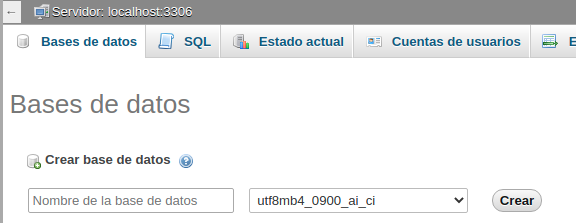
\includegraphics[width=0.9\textwidth]{logos/menubd1.png}\\[1.4cm]
\caption{Pestaña de creación de base de datos en phpMyAdmin}
\label{img:menubd1}
\end{figure}

Una vez creada la base de datos, navegaremos hacia ella a través de la interfaz gráfica y pulsaremos sobre el botón \textbf{Importar} del menú superior de phpMyAdmin. En esta ventana, podremos importar fácilmente el archivo con extensión \textit{.sql} aportado por el tutor de la asignatura, como se muestra en la figura \ref{img:menubd2}. Una vez cargado el script, presionaremos sobre el botón \textbf{Continuar} situado al pie de dicha página, y acto seguido tendremos disponible nuestra base de datos, con todas las tablas y con todos los datos correspondientes.

\begin{figure}[h]
\centering
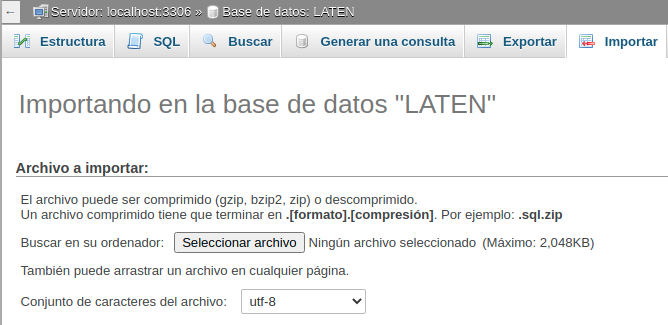
\includegraphics[width=0.9\textwidth]{logos/menubd2.png}\\[1.4cm]
\caption{Pestaña de importación en phpMyAdmin}
\label{img:menubd2}
\end{figure}


\section{Configuración y entorno de JADE}

Como se explicó en la sección \ref{sec:jade}, JADE es un framework que actuará de middleware entre nuestro sistema de agentes.\\

Su configuración es bastante sencilla. En la ya mencionada asignatura, se nos proporcionó un fichero comprimido que contiene todo lo necesario para la instalación de JADE. Con la siguiente secuencia de comandos, instalaremos de manera muy sencilla el paquete:

\begin{lstlisting}
    unzip dba-jade-kit.zip
    cd bin
    sudo ./install.sh
\end{lstlisting}

Una vez instalado, podemos ejecutar el servicio de JADE haciendo uso del siguiente comando:

\begin{lstlisting}
    sudo ./doJade.sh start
\end{lstlisting}

y de igual forma, cambiando el argumento, para detener el servicio:

\begin{lstlisting}
    sudo ./doJade.sh stop
\end{lstlisting}

Estas herramientas que acabamos de instalar también gozan de una interfaz gráfica desde la que observar todos los agentes que se encuentran disponibles en la plataforma además de las comunicaciones que se realizan entre ellos. Para ejecutar dicha interfaz gráfica, usaremos el siguiente comando:

\begin{lstlisting}
    sudo ./doJadeGUI.sh 
\end{lstlisting}

El cual, tras unos instantes nos mostrará una pantalla como la que se muestra en la figura \ref{img:jade1}.

\begin{figure}[h]
\centering
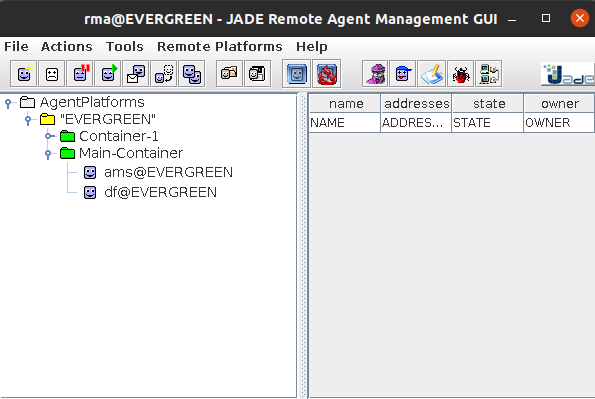
\includegraphics[width=0.9\textwidth]{logos/jade1.png}\\[1.4cm]
\caption{Interfaz gráfica de JADE}
\label{img:jade1}
\end{figure}

\section{Configuración del agente}

Para que nuestro agente se integre de manera correcta en la red con el resto de agentes que ya habitan en ella, es necesario especificar ciertos parámetros de configuración que posteriormente serán leídos por las clases correspondientes que lanzan dicho agente a la plataforma JADE. Estos parámetros de configuración se establecerán en formato JSON, dentro de una carpeta llamada \textit{config} del mismo proyecto de nuestro agente LATEN.\\

Dichos parámetros de configuración son los que se muestran a continuación:

\begin{lstlisting}
    {
        "name": "LATEN",
        "version": "1.0",
        "silent": false,
        "log": true,
        "system": true,
        "showbehaviour": false,
        "singlebehaviour": true,
        "boot": "jade",
        "jadeconnection": {
            "host": "localhost",
            "port": 1099
        },
        "dbconnection": {
            "host": "localhost",
            "port": 3306,
            "database": "LATEN",
            "user": "username",
            "password": "password"
        }
    }
\end{lstlisting}

A destacar de este archivo de configuración, podemos ver el elemento \textbf{singlebehaviour}, el cual tiene como valor asignado \textit{true}, lo cual indica que dicho agente tiene un solo comportamiento y por tanto no es necesario establecer configuraciones adicionales a la hora de lanzar dicho agente, como por ejemplo sería establecer un sistema de colas múltiple para la recepción de mensajes ACL.\\

Otros elementos como \textbf{silent}, \textbf{log} o \textbf{system}, tienen como propósito informar al desarrollador sobre los distintos acontecimientos durante la ejecución de dicho agente. Se pueden configurar a \textbf{true} o \textbf{false} para ajustar la cantidad de información que queremos recibir de la ejecución.\\

Adicionalmente, tenemos un elemento de configuración de la conexión de JADE llamado \textbf{jadeconnection}, en el que podemos especificar el \textbf{host} y el \textbf{puerto \textit{(port)}} a través de los cuales se puede establecer una conexión con JADE.\\

Por último, tenemos el elemento \textbf{dbconnection} que posee toda la configuración necesaria para establecer conexión con la base de datos previamente configurada.

\section{Implementación}

\subsection{Agente LATEN}

El agente LATEN en un inicio se planificó como el agente encargado de interactuar con el resto de los agentes de la red, haciendo de puente entre aquellos agentes destinados a la resolución de las prácticas, como los ya mencionados \textbf{WorldManagers} y entre el propio bot de Telegram.

\subsubsection{Clase principal}

En todo el ecosistema ya mencionado, los agentes se lanzan a la plataforma esencialmente de la misma forma, con quizás algunos cambios. Se puede apreciar en el siguiente fragmento de código, en el que explicaré brevemente en qué consiste cada línea.

\begin{lstlisting}
    static ConsoleBoot _app;

    public static void main(String[] args) {
        _app = new ConsoleBoot("LATEN", args);
        _app.selectConnection();
        _app.launchAgent(LATEN.class);
        _app.shutDown();
    }
\end{lstlisting}

Para comenzar, creamos un objeto de clase de la clase \textbf{ConsoleBoot}, la cual es una clase creada por el profesor de la asignatura para ejecutar aplicaciones JADE con todo lo necesario para que los agentes se puedan ejecutar \textbf{(y ser cerrados)} de manera segura ya sea en nuestra máquina local o en remoto.\\

El siguiente método \textbf{selectConnection()}, selecciona la conexión que hayamos definido en nuestro archivo de configuración JSON, ya sea nuestra máquina local o una máquina remota, como podría ser el propio servidor de la asignatura para realizar las propias prácticas.\\

\textbf{launchAgent()} básicamente lanza al agente a la plataforma y el método \textbf{shutDown()} cerrará el agente junto con los contenedores creados cuando el método \textbf{plainExecute()} de la clase \textbf{LATEN} termine de ejecutarse y por tanto haya finalizado el trabajo del agente.

\subsubsection{El método plainExecute()}

Este es el método principal de la clase \textbf{LATEN}. Es el que se ejecutará durante toda la vida útil del agente. El propósito actual de dicho agente es el de leer, interpretar y actuar sobre los distintos registros de las sesiones prácticas de la asignatura. Al comienzo de este proyecto, el tutor me facilitó los registros reales de las prácticas del grupo de prácticas al que yo pertenecía durante la asignatura, los cuales usé para poder implementar y probar esta funcionalidad.\\

Al lanzar el agente LATEN a la plataforma, para proceder a la lectura e interpretación de los registros, se siguen los siguientes pasos:\\

\begin{enumerate}
    \item Identificar el grupo al que pertenece dicho registro
    \item Identificar los miembros de dicho grupo
    \item Obtener los ajustes de noticaciones específicos de cada usuario del grupo
    \item Analizar cada línea y enviar los mensajes correspondientes al agente de Telegram para que éste informe a los miembros correspondientes
\end{enumerate}

Los tres primeros puntos de la lista anterior se pueden observar, de manera breve en el siguiente fragmento de código:

\begin{lstlisting}
    // Identify which group does this communication belong to
    this.group = this.identifyGroup(myReader.nextLine());
    
    // Verify which members do we have to send the message to
    // First, obtain the groupID
    JsonObject groupID = _dataBase.queryJsonDB("SELECT groupID FROM LATEN.Groups WHERE alias='" + this.group + "'").getRowByIndex(0);
    
    // Members belonging to that group
    JsonArray usersID = _dataBase.queryJsonDB("SELECT userID FROM GroupMembers WHERE cardID IS NOT NULL AND groupID=" + groupID.get("groupID")).getAllRows();
    
    for(int i = 0; i < usersID.size(); i++) {
        this.groupMembers.add(usersID.get(i).asObject());
    }
    
    // Adds the notifications settings for each user
    for(JsonObject groupMember : this.groupMembers) {
        JsonObject usersNotifications = 
                _dataBase.queryJsonDB("SELECT notificationSettings FROM Users WHERE userID=" + groupMember.get("userID")).getRowByIndex(0);
        
        groupMember.add("notificationSettings", usersNotifications.get("notificationSettings"));
    }
\end{lstlisting}

Como se puede observar, se realizan varias consultas a la base de datos y estos datos se van almacenando en ciertas variables de la clase para su posterior uso.\\

Con respecto al último punto, al comienzo del método se declaran las siguientes variables, que sirven para abrir y leer el archivo correspondiente de las sesiones:

\begin{lstlisting}
    File ficheroSesiones = new File(sessionFile);
    Scanner myReader = new Scanner(ficheroSesiones);
\end{lstlisting}

De tal forma, una vez se hayan hecho todas las consultas necesarias a la base de datos y almacenado los datos correspondientes, podremos iterar sobre cada línea del registro con un bucle y así analizar y actuar sobre cada línea:

\begin{lstlisting}
    while(myReader.hasNextLine()) {
        String linea = myReader.nextLine();
        
        JsonObject jsonLine = Json.parse(linea).asObject();
        String info;
        
        if (linea.contains("acl_receive_REGULAR") && linea.contains("\"command\":\"login\"")) {
            // This is a notification marked as ALL
            String newConvIDs = this.buildNotificationString("ALL");                
            
            sendMessage("PTelegram", ACLMessage.AGREE, "REGULAR", Emojis.ENVELOPE + " Sending login request...", newConvIDs);
            
        } else if (linea.contains("acl_send_REGULAR") && linea.contains("Login request from")) { [...]
\end{lstlisting}

\subsubsection{Métodos auxiliares}

En el método \textbf{plainExecute()} se han podido observar otras funciones auxiliares que se programaron para modularizar lo máximo posible el agente y hacerlo así más legible, y sobre todo más mantenible de cara a un futuro. A continuación se comentan las más relevantes:\\

La primera que procedo a comentar es quizás la más destacable y la más usada, ya que en cada condición diferente del bucle principal del método \textbf{plainExecute()} se usa. Es la función encargada de mandar un mensaje a un determinado agente de la plataforma. Recibe ciertos parámetros como el nombre del agente, la performativa a enviar, o el contenido, como se puede observar a continuación:\\

\begin{lstlisting}
    /**
     * Sends a message
     * @param receiver Message's receiver
     * @param performative The performative to use
     * @param protocol Message's protocol
     * @param content Message's content
     * @param conversationID The conversation ID to send the message to
     */
    protected void sendMessage(String receiver, int performative, String protocol, String content, String conversationID) {
        ACLMessage out = new ACLMessage();
        out.setSender(this.getAID());
        out.addReceiver(new AID(receiver, AID.ISLOCALNAME));
        out.setPerformative(performative);
        out.setProtocol(protocol);
        out.setContent(content);

        if(conversationID != "") {
            out.setConversationId(conversationID);
        }

        this.send(out);
    }
\end{lstlisting}

Como observamos en la función anterior, es necesario proveer de un \textit{conversationID}, que es esencialmente una cadena de caracteres, que puede estar separada por espacios, en la que se indica cada uno de los chats a los que se les debe entregar cada mensaje. Así pues, en la siguiente función lo que se hace es constuir esa cadena de caracteres en base a las preferencias de notificaciones de cada usuario:\\

\begin{lstlisting}
    /**
     * Returns an updated list of conversation IDs to send the notifications
     * @param notification rank
     * @return String containing the conversation IDs
     */
    protected String buildNotificationString(String notification) {
        String convIDs = "";
        
        for (JsonObject groupMember : this.groupMembers) {
            for (String type : notification.trim().split(" ")) {
                if (groupMember.get("notificationSettings").toString().replaceAll("\"", "").equals(type)) {
                    convIDs = convIDs + " " + groupMember.get("userID").toString();
                }
            }
        }
        
        return convIDs;
    }
\end{lstlisting}

De tal modo, en la siguiente línea se especifica que se debe enviar ese mensaje concreto, a aquellos usuarios que tengan las preferencias de notificaciones en \textit{''ALL''}:\\

\begin{lstlisting}
    // This is a notification marked as ALL
    String newConvIDs = this.buildNotificationString("ALL");
\end{lstlisting}

Como ya se ha comentado en otras ocasiones, debido a falta de tiempo y otros diversos problemas, no se ha podido proceder al lanzamiento de este agente a la plataforma con el resto de agentes de la asignatura. Se comentarán más detalles en la sección de trabajos futuros.

\subsection{Agente PTelegram \textit{(Public Telegram)}}

El agente correspondiente al proyecto PTelegram, denominado de igual forma en la plataforma de agentes, es aquel que se encargará esencialmente de procesar todas las actualizaciones que lleguen tanto de Telegram como a través de mensajes provenientes de otros agentes en la red. Este proyecto parte del proyecto inicialmente desarrollado por el profesor, llamado \textbf{PublicTelegram}, y el motivo por el que crear uno idéntico a ese y renombrarlo a \textbf{PTelegram} fue esencialmente por facilidad a la hora del desarrollo, tal y como sugirió el tutor del proyecto.\\

Este agente hereda del agente \textbf{BaseTelegram}, que proporciona funcionalidad abstracta para su posterior implementación. El motivo de tener esta clase padre, es que en la asignatura existen dos tipos de bots de Telegram: el bot destinado a los alumnos \textit{(PublicTelegram)} y el bot destinado al profesor \textit{(PrivateTelegram)}.

\subsubsection{Clase principal}

Como podemos observar en el siguiente fragmento de código, la manera de inicializar el agente perteneciente a \textit{PTelegram} es prácticamente idéntica a la del agente \textit{LATEN}. La única diferencia, obviamente, es el nombre que se le pasa como parámetro al crear el objeto de la clase \textbf{ConsoleBoot}:\\

\begin{lstlisting}
    public static void main(String[] args) {
        ConsoleBoot app = new ConsoleBoot("AgentTelegram", args);
        app.selectConnection();
        app.launchAgent(PublicTelegram.class);
        app.shutDown();
    }
\end{lstlisting}

\subsubsection{El método plainExecute()}

Como se ha mencionado anteriormente, la clase \textbf{PTelegram} hereda de \textbf{BaseTelegram}, y por lo tanto esta clase hija no tiene un método \textit{plainExecute()} definido, si no que usará por defecto el de la clase padre.\\

Es importante diferenciar entre dos tipos de actualizaciones que le llegaran al agente. En primer lugar, tenemos las actualizaciones que llegan evidentemente desde cada chat de Telegram. Esto es, cuando un usuario utiliza cualquiera de los comandos operativos en el mismo. Además, tenemos las actualizaciones provenientes del resto de agentes de la red y más concretamente para este proyecto, aquellos mensajes que son enviados desde nuestro agente \textbf{LATEN} hacia el agente \textbf{PTelegram} para proceder a la difusión de mensajes en los chats correspondientes.\\

Por tanto, la misión del método \textit{plainExecute()}, que recordemos que se ejecuta \textit{''indefinidamente''}, será la de comprobar periódicamente si existen actualizaciones de cualquiera de los dos tipos mencionados y procesarlas como sea necesario:\\

\begin{lstlisting}
    @Override
    public final void plainExecute() {
        Update u; // Cola de mensajes de Telegram (Telegramchat)
        ACLMessage iu; // Cola de mensajes de LARVA blockingReceive()
    
        // Process one single update for every queue, to do a kind of leveled answer to all inbound requirements
        for (long cid : telegramQueue.getAllChatIDActive()) {
            u = telegramQueue.popUpdateChatID(cid);
            processTelegramUpdate(cid, u);
        }
        
        // Internal updates
        this.processACLMUpdates();
        if (this.internalUpdates.size() > 0) {
            iu = this.internalUpdates.get(0);
            this.internalUpdates.remove(0);
            processInternalUpdate(iu);
        }
        
        // Wait for a little while
        if (telegramQueue.isAllEmpty() && this.internalUpdates.isEmpty()) {
            doBlock(500);
        }
    }
\end{lstlisting}

Los dos método que se llaman en este método, \textit{processTelegramUpdate} y \textit{processInternalUpdate} son métodos abstractos de la clase \textbf{BaseTelegram} que deberán ser implementados ya sea en \textbf{PTelegram} o en \textbf{PrivateTelegram}.\\

Para comenzar, el método \textit{processTelegramUpdate} implementado en \textbf{PTelegram}, una vez recibe una actualización de un chat de Telegram, verifica que está haciendo uso de uno de los comandos establecidos y ejecuta la función correspondiente, como se puede observar en el siguiente fragmento de código \textit{(incompleto y adaptado a este documento)}:\\

\begin{lstlisting}
    @Override
    protected void processTelegramUpdate(long cid, Update u) {
        if (!isDebug || cid == this.LCastilloCID) {
            TelegramChat tc = this.telegramQueue.getChatData(cid);
            File cardfile;
            if (u.getMessage().hasText()) {
                String line = u.getMessage().getText(), parameters[] = line.split(" ");
                switch (parameters[0]) {
                    case "/help":
                        this.sendTelegram(cid, help(cid));
                        break;
                        
                    case "/notificationstatus":
                        doCheckNotificationsStatus(cid);
                        break;
                        
                    case "/myprogress":
                        doMyProgress(cid);
                        break;
                        
                    default:
                        this.sendTelegram(cid, hello);
        [...]
\end{lstlisting}

Por último, el método \textit{processInternalUpdate} actúa de manera similar. Tras unas comprobaciones iniciales, procede a comprobar qué performativa recibe del mensaje correspondiente y así realizar las accioens necesarias \textit{(fragmento de código incompleto y adaptado a este documento)}:\\

\begin{lstlisting}
    @Override
    protected void processInternalUpdate(ACLMessage msg) {
        ArrayList<Long> usersinvolved = new ArrayList();
        String what, convid = "";
        JsonObject jsreport;

        try {
            [...]
            switch (msg.getPerformative()) {
                case ACLMessage.REQUEST:
                    [...]
                    break;
                case ACLMessage.INFORM:
                    [...]
                    break;
                case ACLMessage.AGREE:
                    [...]
                    break;
            }
            
        [...]
\end{lstlisting}

\subsubsection{Métodos auxiliares}

Con respecto al resto de métodos auxiliares, en concreto para el método \textit{processTelegramUpdate}, se implementan en la propia clase \textbf{BaseTelegram} y se usa uno distinto para cada comando recibido a través de Telegram. Los más complejos requieren de algunas consultas a la base de datos.\\

Por poner un ejemplo, ya que algunos además de consultas a la base de datos requieren de algunos cálculos y comprobaciones adicionales, a continuación se muestra el método \textbf{doSetNotifications()}, que se llama cuando desde Telegram se recibe el comando \textit{/notifications <option>}. Desde la clase \textbf{PTelegram} se comprueba que los parámetros son correctos, y en tal caso, se llama al método \textbf{doSetNotifications()} que actualiza en la base de datos las preferencias de notificaciones del usuario de dicho chat.\\

Una vez hechas las consultas, se envía el mensaje correspondiente al chat del usuario. Un ejemplo del funcionamiento se puede visualizar en la figura \ref{img:exampletelegram}.

\begin{lstlisting}
    protected void doSetNotifications(long cid, String type) {
        TelegramChat tc = this.telegramQueue.getChatData(cid);
        
        try {
            _dataBase.updateDB("UPDATE Users SET notificationSettings='" + type + "' WHERE userID='" + tc.getUserID() + "'");
            this.sendTelegram(cid, Emojis.INFO + " Notifications set to " + type);
        } catch (Exception ex) {
            Exception("", ex);
            this.sendTelegram(cid, Emojis.WARNING + "I could not perform this task due to an internal error. Please try later");
        }
    }
\end{lstlisting}

\begin{figure}[h]
\centering
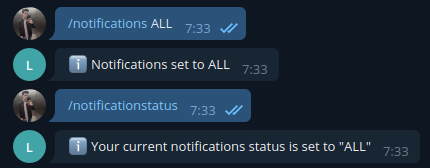
\includegraphics[width=0.9\textwidth]{logos/exampletelegram.png}\\[1.4cm]
\caption{Ejemplo del funcionamiento de los comandos \textit{/notifications <option>} y \textit{/notificationstatus} en el bot LATEN de Telegram}
\label{img:exampletelegram}
\end{figure}

\subsection{Resto de clases y utilidades}

Además de los proyectos mencionados \textit{(LATEN, PTelegram y BaseTelegram)}, estos se valen de otros proyectos adicionales que han sido desarrollados por el profesor de la asignatura y que simplemente me gustaría comentar para contextualizar este proyecto, a pesar de que no han sido modificados en el ámbito de este proyecto.\\

En la siguiente lista se muestran algunas de las utilidades que considero más importantes:

\begin{itemize}
	\item Paquete \textbf{AdminKeys \textit{(en el proyecto CoreLARVAAdminObjects)}}: Implementa ciertas utilidades para la encriptación \textit{(y desencriptación)} de las ya mencionadas cardIDs
	\item Paquete \textbf{Database \textit{(en el proyecto CoreLARVAAdminObjects)}}: Todas las herramientas para poder hacer consultas a la base de datos
	\item Paquete \textbf{ControlPanel \textit{(en el proyecto CoreLARVAAgents)}}: Proporciona a los estudiantes a tener un panel de control visual para el desarrollo de las prácticas
	\item Paquete \textbf{Map2D \textit{(en el proyecto CoreLARVAMoreObjects)}}: Es el que visualmente, junto con el paquete \textbf{ControlPanel}, hace que se visualicen correctamente los mapas de las prácticas de la asignatura
\end{itemize}

Son más las utilidades que se proporcionan y que demuestran que ha sido un trabajo laborioso, largo y cuidado por parte del profesor de la asignatura.

\section{Diagrama de clases}

\section{Ejemplo de comunicación entre agentes}

\section{Control de versiones: git y GitHub}

Además de las herramientas de desarrollo previamente mencionadas en las secciones de este capítulo, se han usado además otras dos herramientas para facilitar el desarrollo.\\

En concreto, para tener un control de las distintas versiones del proyecto, tanto a nivel de código como a nivel de documentación, he usado \textit{git} como tecnología de control de versiones y \textit{GitHub} para almacenar todo el proyecto.\\

El motivo de usar control de versiones surge desde el comienzo de mis estudios en el grado de Ingeniería Informática, donde se me presentó la necesidad de almacenar mis proyectos en un lugar seguro para evitar posibles pérdidas y además poder volver a versiones anteriores del código por si en algún momento del desarrollo algún componente falla, o se introduce algún fragmento de código que hace dejar de funcionar otra parte de manera estrepitosa.\\

Así, esa necesidad siguió evolucionando y siendo implementada de mejor manera por mi parte de lo largo del grado hasta llegar a este proyecto. Debido a la naturaleza del proyecto y que contiene algunos fragmentos de código sensibles que los alumnos de la asignatura no deberían tener accesibles, el repositorio de GitHub no se hará público, decisión que se tomó en consenso con el tutor de este proyecto.\\

No obstante, personalmente he mantenido de manera natural el control de versiones mediante el repositorio de GitHub como si fuese otra asignatura o proyecto más, a pesar de que no se hará público, al menos por ahora.